\chapter{提案手法の概要}
関連研究の章ではニューラルネットワークや決定木が内包する説明性の欠如という問題点と説明を加える既存手法の持つ課題について述べた.
本論文ではそれらを踏まえた
\begin{itemize}
	\item 本来ゲームに存在する時系列の要素を含む
	\item 評価基準が勝敗に直結する
    \item 人間のドメイン知識に依存しない
\end{itemize}
説明手法を提案する.
図\ref{fig:mabs}に提案手法の概要を示している.
本手法はある状態$s$と行動$a$の組に対してAIが予想する未来図$O(s)$とそこに至るまでの道筋の集合を取り出し,その傾向を見出すことによるAIの判断
の意図を可視化を目標とする.
以降は未来図$O(s)$と走査が$O(s)$に至るまでに通過したノードの履歴(軌道)$\zeta(s, O(s))$を合わせて進行図と記載する.
\begin{figure}[t]
    \centering
    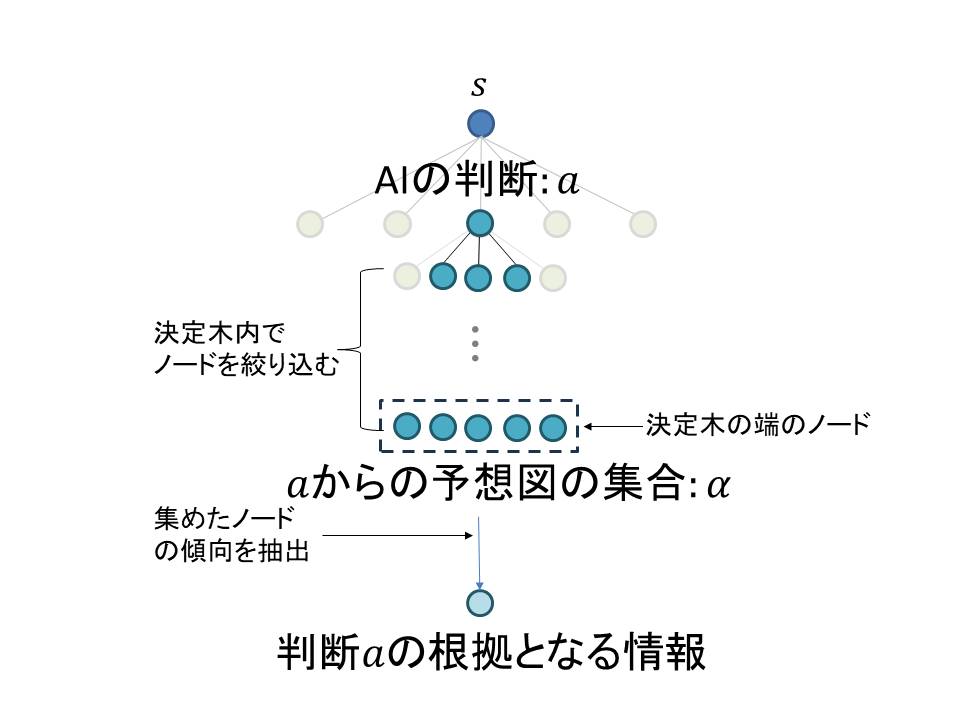
\includegraphics[width=\linewidth]{./figure/mabs.png}
    \caption{提案手法の概要}
    \label{fig:mabs}
\end{figure}
本章では提案手法のアルゴリズムと,第2章で述べた重要度$I(s)$の新たな定義を記載する.
それから,
実験のタスクとして選択したconnect4と使用したモデルであるalphazero\_baseline,提案手法のconnect4への応用例について記載する.


\section{提案手法のアルゴリズム}
本手法はAlphaZeroシステムのニューラルネットワークと木探索部分のうち,主に木探索の部分を対象に適用される.
本手法では決定木の判断を説明する際に最も有用な部分を決定木から抽出することを主な目的としており,アルゴリズムはボードゲームAIに留まらず決定木構造を持つ多くのシステムに応用可能である.
アルゴリズムの流れは以下の通りである.
図\ref{fig:step1-2},図\ref{fig:step3-4}はステップごとのアルゴリズムのイメージ図である.
\begin{enumerate}
    \item 説明を付与する状態と行動の組$(s_{start}, a)$を選択する.
    このとき注目している状態$s_{now}, a_{now}$はそれぞれ
    \begin{equation}
        {s_{now}=s_{start}}
    \end{equation}
    \begin{equation}
        {a_{now}=a}
    \end{equation}
    とする.
    \item 以下の流れを$l$ステップ分繰り返す.\\
    決定木中の注目しているノード$s_{now}$における訪問回数$N(s_{now})$中の上位$k$個分の行動$\{a_1, a_2, ..., a_{k}\}(a_iはk番目に有望な行動とする)$を取り出す.
    $s_{now}$から行動$\{a_1, a_2, ..., a_{k}\}$を取ることでたどり着く各ノード\\
    $\{s_{next_1}, s_{next_2}, ..., s_{next_{k}}\}(s_{next_i}=T(s_{now}, a_i), Tは遷移関数)$に対して同様の操作を繰り返す.
    
    
    \item 集めた$k$の$l$乗個のノード$\{{s}'_{1}, {s'}_{2}, ..., {s'}_{k^l}\}$のそれぞれ${s'}_{i}(i=1, 2, ..., k^l)$に対して以下の操作を再帰的に繰り返す.
    ${s'}_{i}$における方策$P({s'}_{i})$中の最も有望な行動$a_{promising}$と${s'}_{next_i}=T({s'}_i, a_{promising})$を記録する.
    そのようにして記録した$\{{s'}_{next_1}, {s'}_{next_2}, ..., {s'}_{next_{k^l}}\}$のそれぞれ${s'}_{next_j}(j=1, 2, ..., k^l)$にも同様の操作を盤面ノードが決定木の端に辿り着くまで行う.
    \item step3によってたどり着いた$k^l$個のノードによる集合$S=\{s_{edge_1}, s_{edge_2}, ..., s_{edge_{k^l}}\}$を任意の共通項$c$によっていくつかの副集合$\{S_1, S_2, ..., S_q\}$に分ける.
    \item 共通項で括られた各集合$\{S_1, S_2, ..., S_q\}$のうち,最も要素数が多いもの$S_{max}$中の各要素$\{s_{e_1}, s_{e_2}, ...,  s_{e_u}\}$と各要素に対応する軌道$\{\rm{{\zeta}_{s_{e_1}}}, \rm{{\zeta}_{s_{e_2}}}, ...,  \rm{{\zeta}_{s_{e_u}}}\}$を抽出する.
    ここでの軌道$\rm{{\zeta}_{s_{e_i}}}$とは,図\ref{fig:traj-example}に示すように決定木を走査する際に$s_{start}$から$s_{e_i}$にたどり着く際に,どのような状態$s$や行動$a$を経由したかを表している.
    図\ref{fig:traj-example}における$\rm{{\zeta}_{s_{e_i}}}$は$\{s_{start}, a_1, s_1, a_2, s_2, a_3, s_3, a_4, s_{e_i}\}$となる.

\end{enumerate}


\begin{figure}[t]
    \centering
    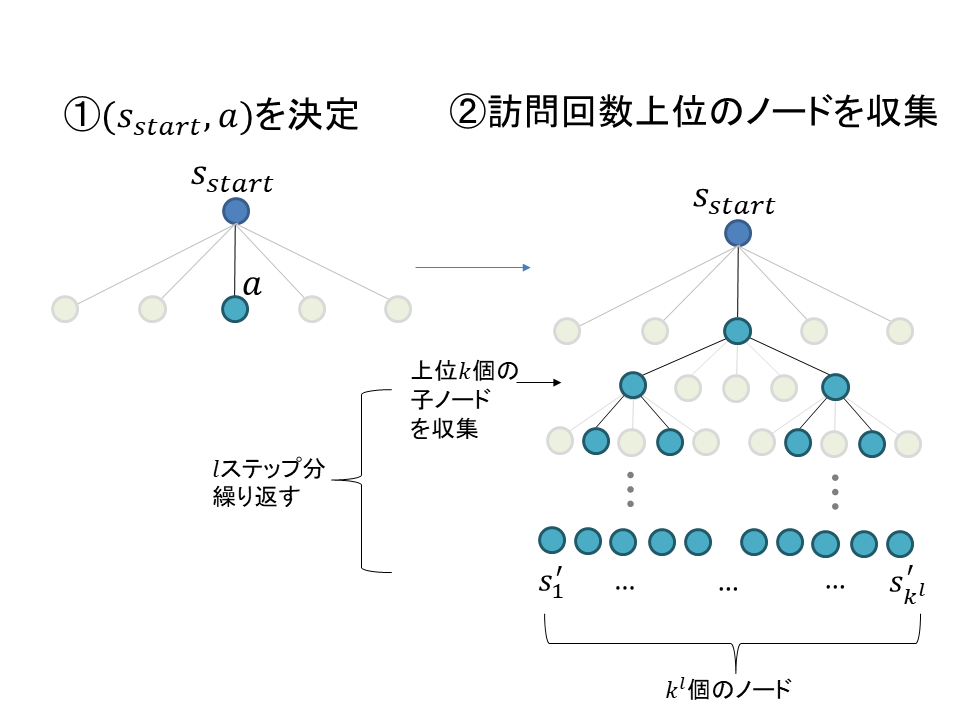
\includegraphics[width=\linewidth]{./figure/1-2.png}
    \caption{提案アルゴリズムの概要(step1$\sim$ 2)}
    \label{fig:step1-2}
\end{figure}
\begin{figure}[t]
    \centering
    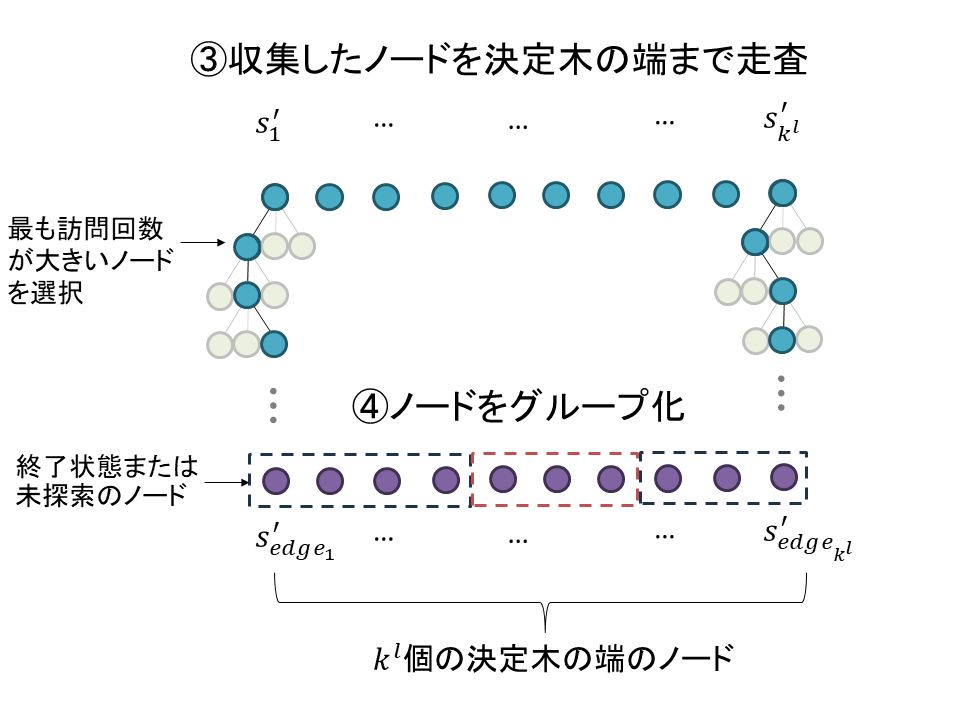
\includegraphics[width=\linewidth]{./figure/3-4.png}
    \caption{提案アルゴリズムの概要(step3$\sim $4)}
    \label{fig:step3-4}
\end{figure}
\begin{figure}[t]
    \centering
    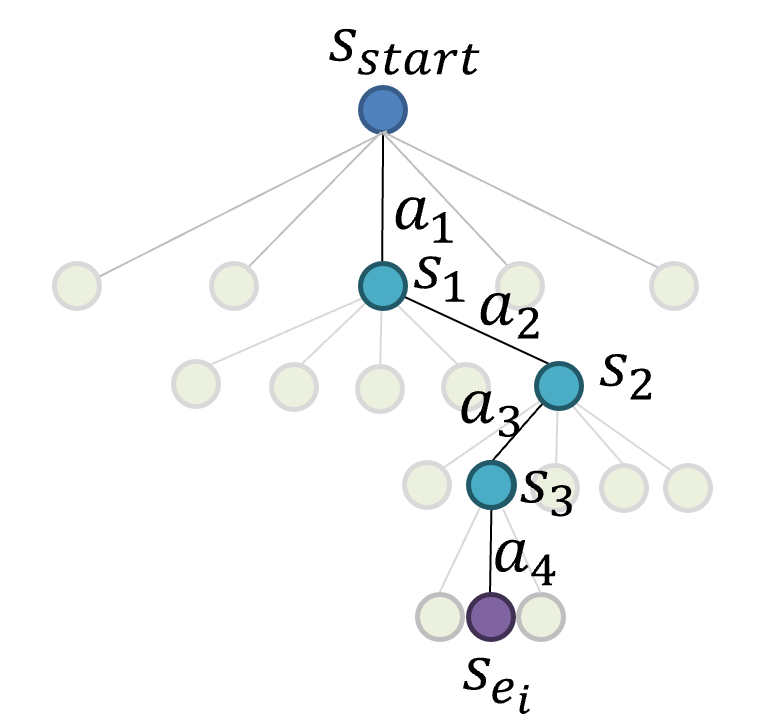
\includegraphics[width=300pt]{./figure/traj-example.png}
    \caption{軌道の例}
    \label{fig:step3-4}
\end{figure}
このアルゴリズムを要約すると,図\ref{fig:merit}のようにある局面$s$と行動$a$の組み合わせから辿り着きやすい結末$O(s, a)$を抽出し,同時に$O(s, a)$に至るまでの複数の道筋を抽出すると表現できる.
調査を行う者が複数の道筋を観察できることで,
共通する傾向や法則性を見出せるというメリットが存在する.これは第2章で述べたような最も可能性が高い1つの分岐を示す,といったような情報が単一である従来の手法には不可能である.
提案手法の疑似コードは付録\ref{chap:alg}に記載している.

\begin{figure}[t]
    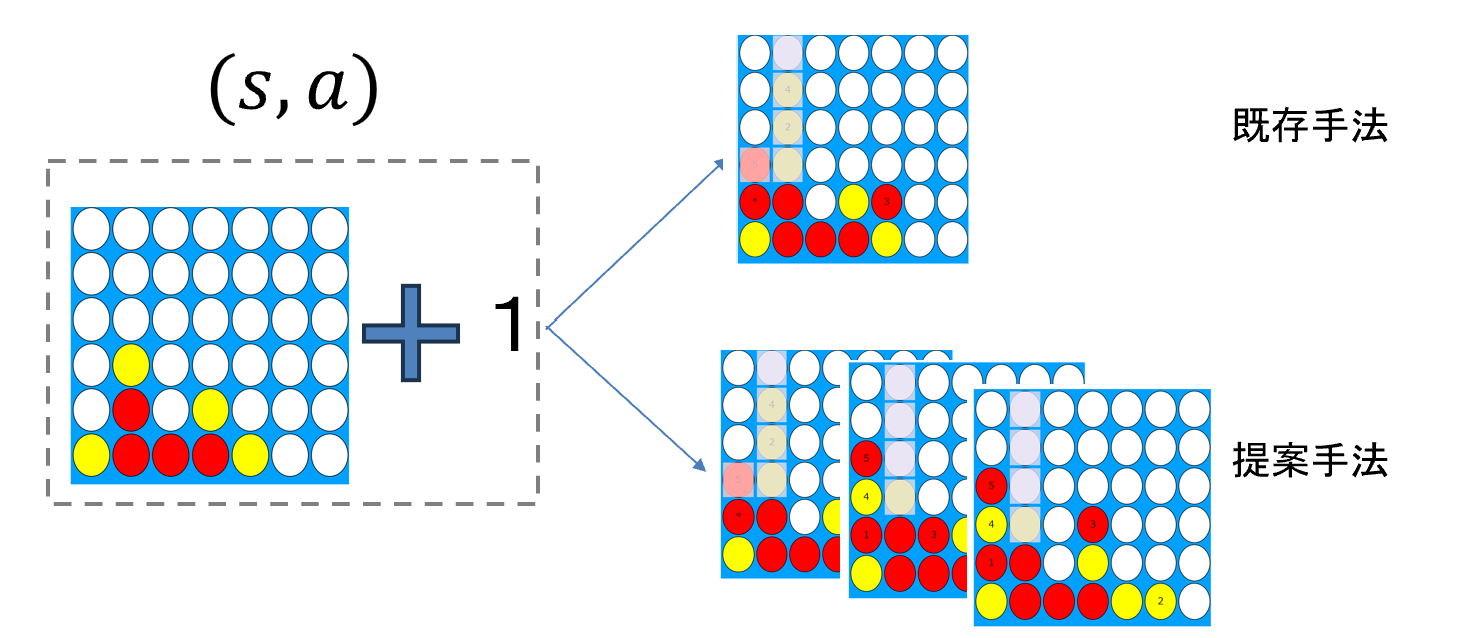
\includegraphics[width=400pt]{./figure/merit.png}
	\caption{提案手法と既存手法}
	\label{fig:merit}
\end{figure}




付録\ref{chap:data}で示すようにconnect4タスクにおいて収集される軌道の集合においては末端部分のいくつかの選択が共通している傾向が確認された.
そのため状態と行動の組$(s, a)$から$O(s, a)$という結果を予測する過程で$O(s, a)$から末尾の数手を取り除いた版面$d$にたどり着く傾向の発見などの知識獲得が記載される.
\section{importance}
前章で述べたように,エピソード中の各状態$s$の重要度$I(s)$の定義を以下のように定めた.
\begin{equation}
    \label{new-imp}
	{I(s)=V[Q'] (Q'=[\rm{max}Q(s, a), \rm{secondMax}Q(s, a), ..., \rm{thirdQuantile}Q(s, a)])}
\end{equation}
つまり,現在の状態$s$に対する行動の集合$A(={a_1, a_2, ..., a_N})$とした際の行動価値関数の集合${Q(s, a_1), Q(s, a_2), ..., Q(s, a_N)}$のうち値の大きさが上位75
\%の成分で構成される集合の分散として重要度$I(s)$を定義する.
これは次の1手で辿り着きうる収益の予想の揺らぎの幅を意味しており,先述した盤面の対称性や悪い選択肢の影響が大きくなる可能性の軽減が期待できる.

\section{connect4}
connect4はボードゲームの一種である.ルールは五目並べに極めて近く,図\ref{fig:connect4}の右側の画像のように,2人のプレイヤーが交互に互いの駒を盤上に置き,最終的に縦,横,もしくは斜めに連続して4つの石を並べたプレイヤーの勝利となる.ただし,五目並べや連珠との相違点として「重力」の存在が挙げられる.
この「重力」とは各プレイヤーが石をボード上の最も下の行または既に置かれた石の上にしか置けないという規則を表している.そのため,各プレイヤーの選択肢はボードの列の数と等しい.
図\ref{fig:connect4}の左側は左から5番目の列を指定した際に,石がボード上の最下の列に置かれる様子を示している.
connect4の一般的なボードの広さは$6\times7$であり$6\times7$のコネクト4については1988年にAllis\cite{allis}により知識ベースの手法による先番勝利が証明された.
Tromp\cite{data}によるconnect4の$\alpha-\beta$木探索によって導かれた各盤面の最善手とそのデータも一般に公開されている.
また,connect4は盤上に全ての情報が開示されており,結果もどちらか一方の勝利または引き分けのみであるため2人ゼロ和完全情報ゲーム\cite{gairon}に分類される.
本論文の実験において提案手法をconnect4に適用する際には最終盤面において4つ以上並んでいる石の座標を特徴として用いた.
\begin{figure}[t]
	\centering
    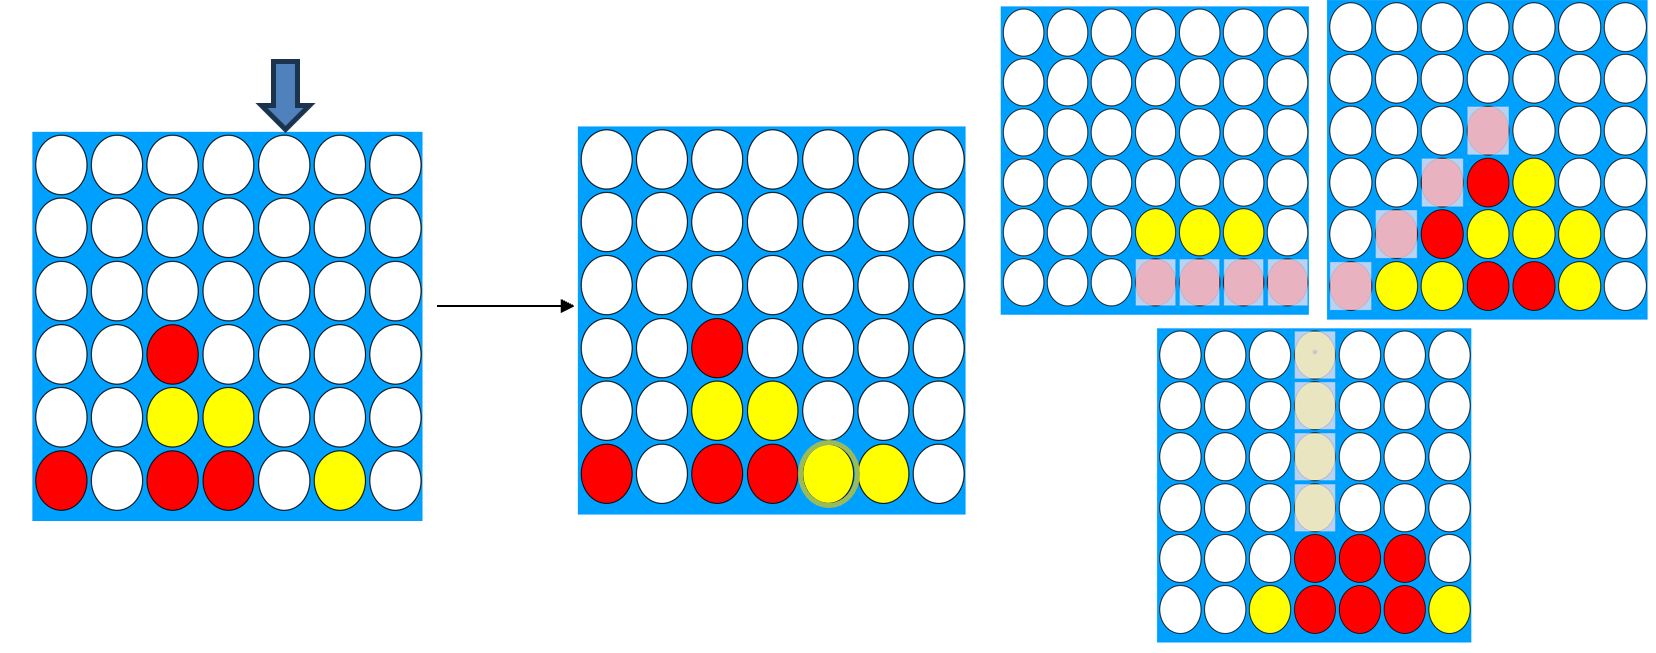
\includegraphics[width=\linewidth]{./figure/connect4.png}
	\caption{connect4}
	\label{fig:connect4}
\end{figure}
\section{alphazero\_baseline}
alphazero\_baselineはalphaZeroをconnect4用に簡易的に模したネットワークであり,図\ref{fig:baseline}に示すように入力は最新の盤面$s_0$,出力は$1\times7$(7はボードの列の数)の方策$P(s)(以下s=s_0とする)$とスカラー値の局面評価$V(s)$(値域は-1から1)である.
方策は確率分布であり,要素の値が大きいインデックスを選択することで勝利に近づくと予想される.
局面評価は第2章の強化学習の段で記載した状態価値関数と同一の変数であり,
入力に対する評価を表しており,1が入力の手番のプレイヤーにとっての勝利,-1が敗北の予想を表している.

\begin{figure}[t]
    \centering
    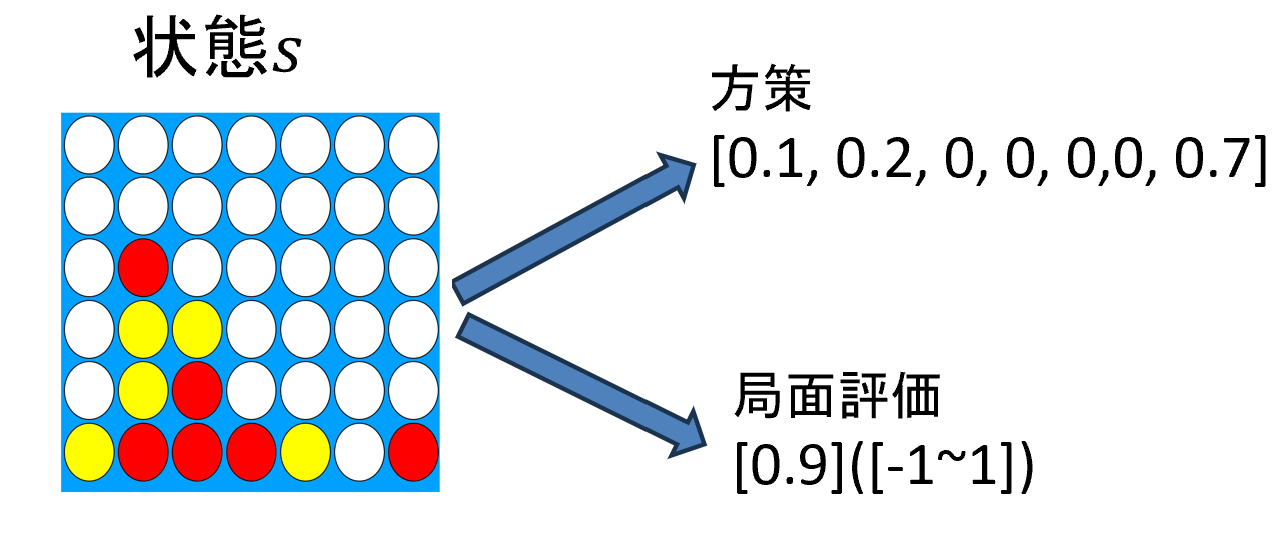
\includegraphics[trim={0cm 0cm 0cm 0cm},clip]{./figure/baseline.png}

    \caption{alphazero\_baselineの入出力}
    \label{fig:baseline}
\end{figure}
\section{提案手法のconnect4への適用}
提案手法をconnect4に適用した際の概要を図\ref{fig:application}に示す.進行図は1組の盤面$s$と行動$a$に対して決定木中の有力なノードを走査することで生成される.
提案手法をconnect4に適用する際,各ノードはalphazero\_baselineへの入力であるconnect4の各盤面となる.

また,ゲームのルールより収集される最終状態では図\ref{fig:application}の下部のように4つ以上並んだ石が存在する.
第4章で詳しく述べるように,実験では4つ以上並んだ石の位置で最終状態をグループ化した.図\ref{fig:application}においては石が左下から右斜め上方向に4つ並んでいる盤面
が最も多いため,赤線で囲われた盤面とそこにいたるまでの軌道が保存される.
\begin{figure}[t]
	\centering
	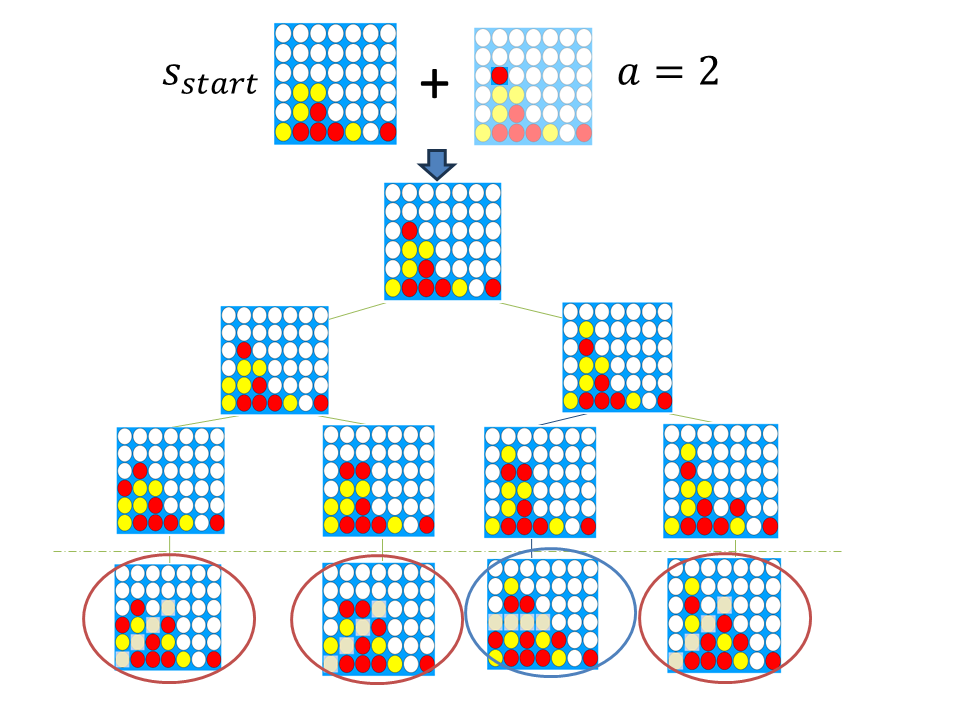
\includegraphics[width=\linewidth]{./figure/application.png}
	\caption{提案手法のconnect4への適用}
	\label{fig:double}
\end{figure}

提案手法により生成される進行図を図\ref{fig:double}に示す.
先述のように進行図は予測図と軌道で構成されている.connect4では盤面$s$と行動$a$を選んだ際の次の状態$s_{next}$は$(s, a)$に対して一意に決定される.
そのため,軌道$\rm{{\zeta}_{s_{e_i}}}$は$s_{start}$から$s_{e_i}$に至るまでに取った行動$a$の集合とした.各行動は選択した列のインデックスで$1\sim7$の数字として
表現される.
\begin{figure}[t]
	\centering
	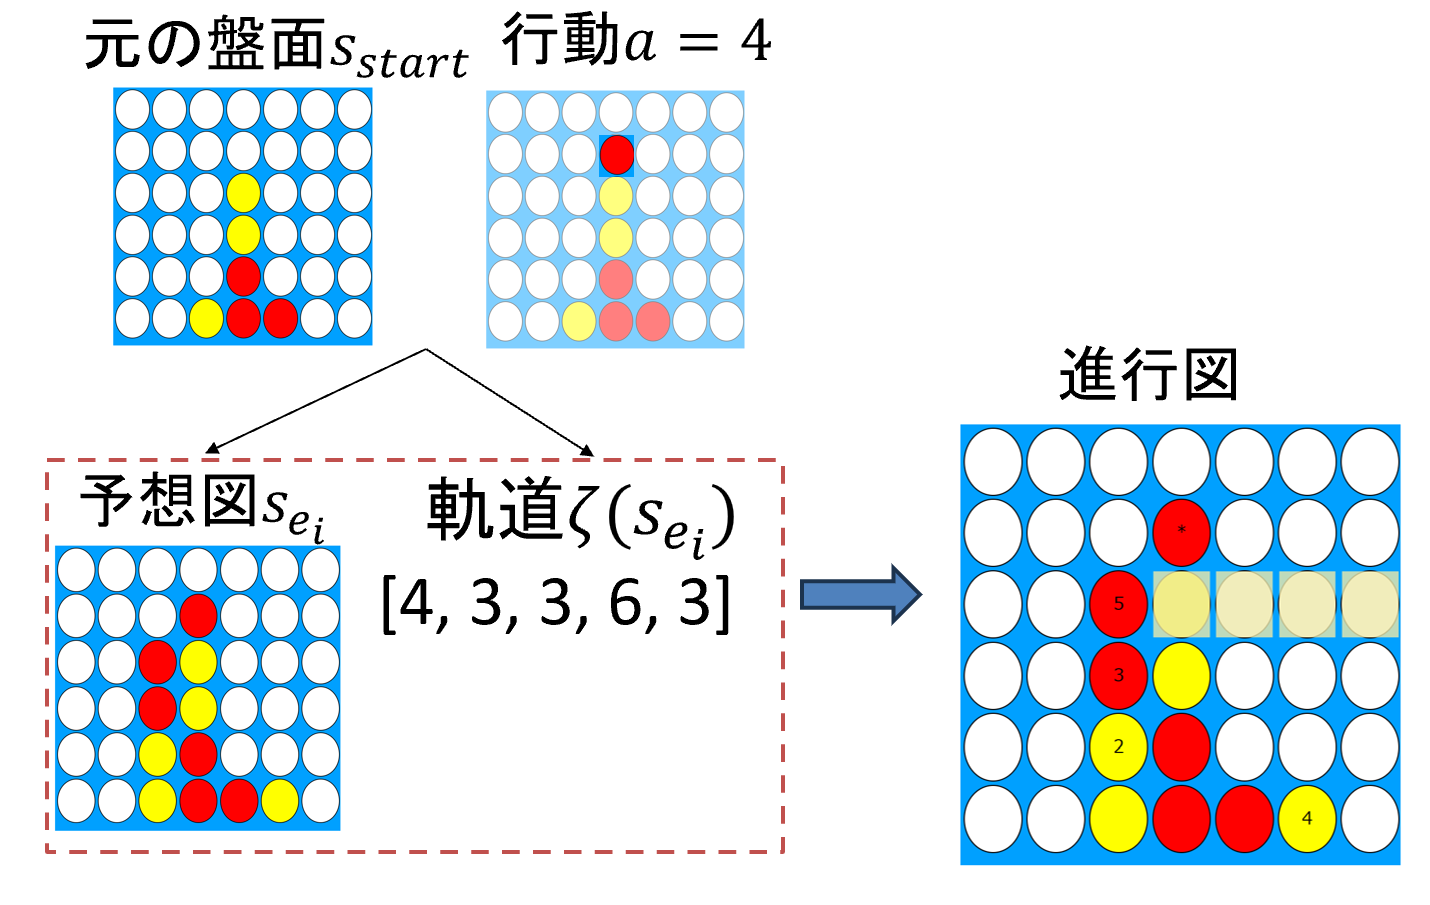
\includegraphics[width=\linewidth]{./figure/double.png}
	\caption{connect4における進行図}
	\label{fig:double}
\end{figure}